\formdesc{Régulation Numérique}

\underline{Théorème  de la valeur final en Z}

valable que si la valeur finale existe et est finie !

$x_\infty = \lim_{z\rightarrow 1} ((z-1)X(z))$

contre-exemple :

$X(z) = \cfrac{z}{z-2} \Rightarrow x[k] = 2^k$

pas fini

\underline{Théorème  de la valeur final en Z}

Décomposer en élément simple :

{\footnotesize
$F(z) = \cfrac{z}{(z+A)(z+B)} \Rightarrow \cfrac{F(z)}{z} = \cfrac{R_1}{z+A} + \cfrac{R_2}{z+B}$

$F(z) =R_1\cfrac{z}{z+A} + R_2\cfrac{z}{z+B}\Rightarrow f[k] = R1\cdot(A)^k+ R1\cdot(B)^k$
}

\hformbar

\formdesc{Système dynamique discret :}

Système discret si signaux entrés et sortis sont discrets.

Système discret est dynamique quand la sortie présente dépend de l'entrée présente et des entrées et sorties passées.

\underline{Système dynamique LTI}

\begin{itemize}
    \item Linéaire : principe de superposition 
    \item Stationnaire(invariant) : Coefficients constants
    \item Causal : pas de dépendance des états future
    \item Au repos à l'instant 0 : condition de départ nul
\end{itemize}

Décrit par sa réponse impulsionnelle : 

Si $u(k) = \Delta(k) + 3 \Delta(k-1) - 2 \Delta(k-2)$ 

$y(k) = g(k) + 3 g(k-1) - 2g(k-2)$ 

donc : 

$g(k)$ est un algorithme 

$Y(z) = G(z) \cdot U(z) \Leftrightarrow y(k) = g(k) * u(k)$


\formdesc{Gain statique }

$ K = G_a(s=0) = G_n(z = 1)$

\formdesc{Erreur statique }

\underline{par le gain statique (s'appliquant à un système):}

correspondance : 

$e_infty = G_{ew}(1) \cdot w_\infty$

Maintien :

$e_infty = G_{ev}(1) \cdot w_\infty$


\underline{par le théorème de la valeur finale (s'appliquant à un signal)}

correspondance : 
\begin{enumerate}
    \item Calculer $G_{ew}(z)$ et vérifier la stabilité
    \item Calculer $W(z) = w_infty \cdot \cfrac{z}{z-1}$
    \item Calculer $E(z) = G_{ew}(z) \cdot W(z)$
    \item Appliquer le théorème : $e_\infty = \lim_{z\rightarrow 1} ((z-1)E(z))$
\end{enumerate}

Condition pour que l'erreur statique correspondance soit nulle :

Soit le système à régler doit avoir un intégrateur pur, soit le régulateur (action I).


Condition pour que l'erreur statique maintien soit nulle :

Soit le système doit avoir un intégrateur pur en amont du point d'introduction de la perturbation.

\underline{Erreur de rampe obligatoirement par valeur final}

correspondance : 
\begin{enumerate}
    \item Calculer $G_{ew}(z)$ et vérifier la stabilité
    \item Calculer $W(z) = pente \cdot \cfrac{z}{(z-1)^2}$
    \item Calculer $E(z) = G_{ew}(z) \cdot W(z)$
    \item Appliquer le théorème : $e_\infty = \lim_{z\rightarrow 1} ((z-1)E(z))$
\end{enumerate}

Condition pour que l'erreur rampe soit nulle :

Minimum 2 intégrateur pur dans la boucle ouverte

\hformbar

\newpage
sook 
\newpage

\formdesc{Transformé en Z}

\begin{figure}[H]
    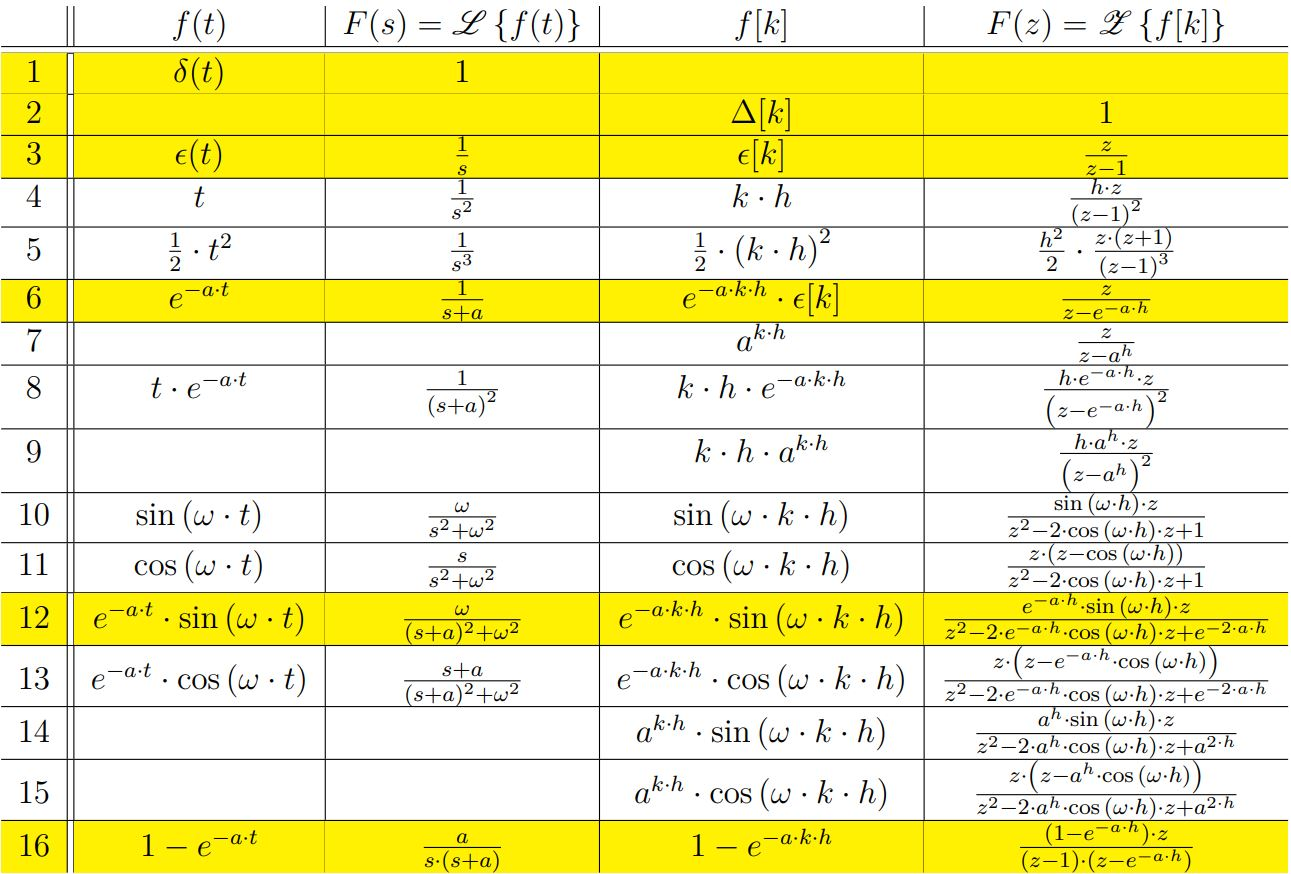
\includegraphics[width  = 1\textwidth]{img/Tranforme_en_Z.JPG}
    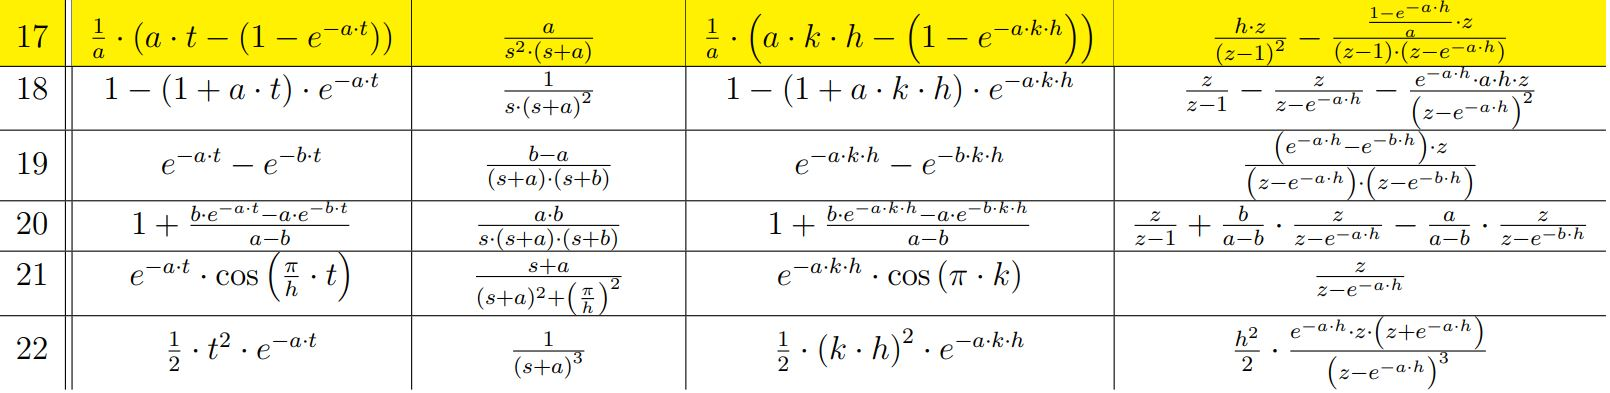
\includegraphics[width  = 1\textwidth]{img/Tranforme_en_Z2.JPG}
\end{figure}